\documentclass{article}
\usepackage[utf8]{inputenc}
\usepackage{tikz}
\usepackage[legalpaper, landscape, margin=1in]{geometry}
\usepackage{geometry}
\geometry{legalpaper, landscape, margin=1in}

\begin{document}

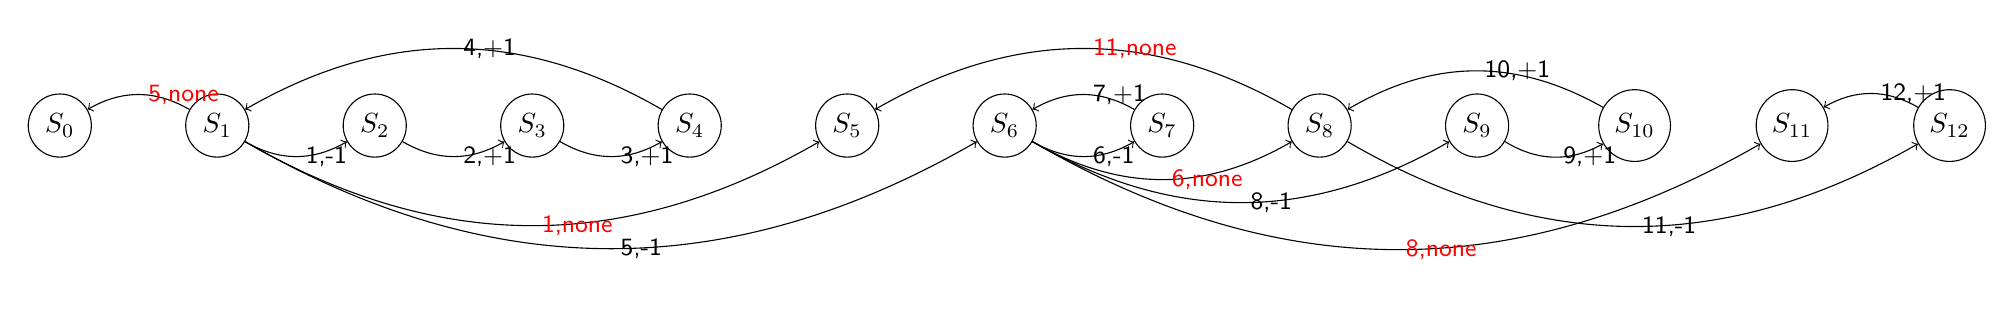
\begin{tikzpicture}[->,node distance={20mm},main/.style = {draw, circle}] 
\node[main] (0) {$S_0$}; 
\node[main] (1) [right of=0] {$S_1$};
\node[main] (2) [right of=1] {$S_2$}; 
\node[main] (3) [right of=2] {$S_3$};
\node[main] (4) [right of=3] {$S_4$}; 
\node[main] (5) [right of=4] {$S_5$};
\node[main] (6) [right of=5] {$S_6$};
\node[main] (7) [right of=6] {$S_7$};
\node[main] (8) [right of=7] {$S_8$};
\node[main] (9) [right of=8] {$S_9$};
\node[main] (10) [right of=9] {$S_{10}$};
\node[main] (11) [right of=10] {$S_{11}$};
\node[main] (12) [right of=11] {$S_{12}$};

 \path[every node/.style={font=\sffamily\small}]
    % 1 (1,-,2,5)
    (1) edge [bend right] node[right] {1,-1} (2)
    (1) edge [bend right] node[right,red] {1,none} (5)
    % 2 (2,+,3)
    (2) edge [bend right] node[right] {2,+1} (3)
    % 3 (3, +, 4)
    (3) edge [bend right] node[right] {3,+1} (4)
    % 4 (4, +, 1)
    (4) edge [bend right] node[right] {4,+1} (1)
    % 5 (3, −, 6, 0)
    (1) edge [bend right] node[right] {5,-1} (6)
    (1) edge [bend right] node[right,red] {5,none} (0)
    % 6 (2, −, 7, 8)
    (6) edge [bend right] node[right] {6,-1} (7)
    (6) edge [bend right] node[right,red] {6,none} (8)
    % 7 (1, +, 6)
    (7) edge [bend right] node[right] {7,+1} (6)
    % 8 (4, −, 9, 11),
    (6) edge [bend right] node[right] {8,-1} (9)
    (6) edge [bend right] node[right,red] {8,none} (11)
    % 9 (5, +, 10)
    (9) edge [bend right] node[right] {9,+1} (10)
    % 10 (2, +, 8)
    (10) edge [bend right] node[right] {10,+1} (8)
    % 11 (5, −, 12, 5)
    (8) edge [bend right] node[right] {11,-1} (12)
    (8) edge [bend right] node[right,red] {11,none} (5)
    % 12 (4, +, 11)
    (12) edge [bend right] node[right] {12,+1} (11)
    
   
 ;
\end{tikzpicture} 
\\
1: $R_1 - 1$ \\
2: $R_2 + 1$ \\
3: $R_3 + 1$ \\
4: $R_4 + 1$ \\
5: $R_3 - 1$ \\
6: $R_2 - 1$ \\
7: $R_1 + 1$ \\
8: $R_4 - 1$ \\
9: $R_5 + 1$ \\
10: $R_2 + 1$ \\
11: $R_5 - 1$ \\
12: $R_4 + 1$ \\
\end{document}